%%%% Paramétrage du TD %%%%
\def\xxactivite{ \ifprof \normalsize{TD 1 -- Corrigé } \else  \ifcolle Colle \else TD 1\fi \fi} % \normalsize \vspace{-.4cm}
\def\xxauteur{\textsl{Xavier Pessoles}}

\def\xxnumchapitre{Chapitre 2 \vspace{.2cm}}
\def\xxchapitre{\hspace{.12cm} Hyperstatisme}



\def\xxcompetences{%
\vspace{-.5cm}
\footnotesize{
\textsl{%
\textbf{Savoirs et compétences :}\\
\vspace{-.2cm}
\begin{itemize}[label=\ding{112},font=\color{ocre}] 
\item \textit{Mod2.C34} : chaînes de solides;
\item \textit{Mod2.C34} : degré de mobilité du modèle;
\item \textit{Mod2.C34} : degré d’hyperstatisme du modèle;
%\item \textit{Mod2.C34.SF1} : déterminer les conditions géométriques associées à l’hyperstatisme;
%\item \textit{Mod2.C34} : résoudre le système associé à la fermeture cinématique et en déduire le degré de mobilité et d’hyperstatisme.
\end{itemize}}}}

\def\xxtitreexo{Interface maître et esclave d'un robot }
\def\xxsourceexo{\hspace{.2cm} \footnotesize{CCP PSI 2015}}

\def\xxfigures{
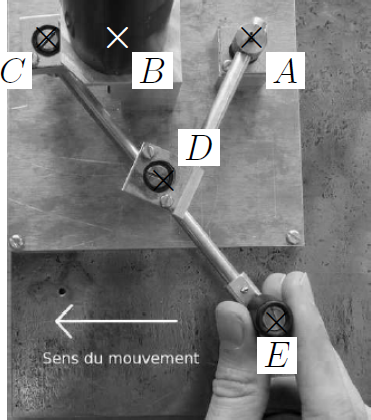
\includegraphics[width=.5\textwidth]{fig_00}
}%figues de la page de garde




\iflivret
\pagestyle{empty}


%%%%%%%% PAGE DE GARDE COURS
\ifcours
% ==== BANDEAU DES TITRES ==== 
\begin{tikzpicture}[remember picture,overlay]
\node at (current page.north west)
{\begin{tikzpicture}[remember picture,overlay]
\node[anchor=north west,inner sep=0pt] at (0,0) {\includegraphics[width=\paperwidth]{\thechapterimage}};
\draw[anchor=west] (-2cm,-8cm) node [line width=2pt,rounded corners=15pt,draw=ocre,fill=white,fill opacity=0.6,inner sep=40pt]{\strut\makebox[22cm]{}};
\draw[anchor=west] (1cm,-8cm) node {\huge\sffamily\bfseries\color{black} %
\begin{minipage}{1cm}
\rotatebox{90}{\LARGE\sffamily\textsc{\color{ocre}\textbf{\xxnumpartie}}}
\end{minipage} \hfill
\begin{minipage}[c]{14cm}
\begin{titrepartie}
\begin{flushright}
\renewcommand{\baselinestretch}{1.1} 
\Large\sffamily\textsc{\textbf{\xxpartie}}
\renewcommand{\baselinestretch}{1} 
\end{flushright}
\end{titrepartie}
\end{minipage} \hfill
\begin{minipage}[c]{3.5cm}
{\large\sffamily\textsc{\textbf{\color{ocre} \discipline}}}
\end{minipage} 
 };
\end{tikzpicture}};
\end{tikzpicture}
% ==== FIN BANDEAU DES TITRES ==== 


% ==== ONGLET 
\begin{tikzpicture}[overlay]
\node[shape=rectangle, 
      rounded corners = .25 cm,
	  draw= ocre,
	  line width=2pt, 
	  fill = ocre!10,
	  minimum width  = 2.5cm,
	  minimum height = 3cm,] at (18.3cm,0) {};
\node at (17.7cm,0) {\rotatebox{90}{\textbf{\Large\color{ocre}{\classe}}}};
%{};
\end{tikzpicture}
% ==== FIN ONGLET 


\vspace{3.5cm}

\begin{tikzpicture}[remember picture,overlay]
\draw[anchor=west] (-2cm,-6cm) node {\huge\sffamily\bfseries\color{black} %
\begin{minipage}{2cm}
\begin{center}
\LARGE\sffamily\textsc{\color{ocre}\textbf{\xxactivite}}
\end{center}
\end{minipage} \hfill
\begin{minipage}[c]{15cm}
\begin{titrechapitre}
\renewcommand{\baselinestretch}{1.1} 
\Large\sffamily\textsc{\textbf{\xxnumchapitre}}

\Large\sffamily\textsc{\textbf{\xxchapitre}}
\vspace{.5cm}

\renewcommand{\baselinestretch}{1} 
\normalsize\normalfont
\xxcompetences
\end{titrechapitre}
\end{minipage}  };
\end{tikzpicture}
\vfill

\begin{flushright}
\begin{minipage}[c]{.3\linewidth}
\begin{center}
\xxfigures
\end{center}
\end{minipage}\hfill
\begin{minipage}[c]{.6\linewidth}
\startcontents
%\printcontents{}{1}{}
\printcontents{}{1}{}
\end{minipage}
\end{flushright}

\begin{tikzpicture}[remember picture,overlay]
\draw[anchor=west] (4.5cm,-.7cm) node {
\begin{minipage}[c]{.2\linewidth}
\begin{flushright}
\includegraphics[width=2cm]{logoCC}
\end{flushright}
\end{minipage}
\begin{minipage}[c]{.2\linewidth}
\textsl{\xxauteur} \\
\textsl{\classe}
\end{minipage}
 };
\end{tikzpicture}

\newpage
\pagestyle{fancy}

%\newpage
%\pagestyle{fancy}

\else
\fi
%% FIN PAGE DE GARDE DES COURS

%%%%%%%% PAGE DE GARDE TD
\iftd

% BANDEAU EXO
\iflivret % SI LIVRET ET TD
\begin{tikzpicture}[remember picture,overlay]
\draw[anchor=west] (-2cm,-3.3cm) node {\huge\sffamily\bfseries\color{black} %
\begin{minipage}{5cm}
\begin{center}
\LARGE\sffamily\color{ocre}\textbf{\textsc{\xxactivite}}

\begin{center}
\xxfigures
\end{center}

\end{center}
\end{minipage} \hfill
\begin{minipage}[c]{12cm}
\begin{titrechapitre}
\renewcommand{\baselinestretch}{1.1} 
\large\sffamily\textbf{\textsc{\xxtitreexo}}

\small\sffamily{\textbf{\textit{\color{black!70}\xxsourceexo}}}
\vspace{.5cm}

\renewcommand{\baselinestretch}{1} 
\normalsize\normalfont
\xxcompetences
\end{titrechapitre}
\end{minipage}};
\end{tikzpicture}
\else % ELSE NOT LIVRET
\begin{tikzpicture}[remember picture,overlay]
\draw[anchor=west] (-2cm,-3.5cm) node {\huge\sffamily\bfseries\color{black} %
\begin{minipage}{5cm}
\begin{center}
\LARGE\sffamily\color{ocre}\textbf{\textsc{\xxactivite}}

\begin{center}
\xxfigures
\end{center}

\end{center}
\end{minipage} \hfill
\begin{minipage}[c]{12cm}
\begin{titrechapitre}
\renewcommand{\baselinestretch}{1.1} 
\large\sffamily\textbf{\textsc{\xxtitreexo}}

\small\sffamily{\textbf{\textit{\color{black!70}\xxsourceexo}}}
\vspace{.5cm}

\renewcommand{\baselinestretch}{1} 
\normalsize\normalfont
\xxcompetences
\end{titrechapitre}
\end{minipage}};
\end{tikzpicture}

\fi

\else   % FIN IF TD
\fi


%%%%%%%% PAGE DE GARDE FICHE
\iffiche
\begin{tikzpicture}[remember picture,overlay]
\node at (current page.north west)
{\begin{tikzpicture}[remember picture,overlay]
\draw[anchor=west] (-2cm,\xxYCartouche) node [line width=2pt,rounded corners=15pt,draw=ocre,fill=white,fill opacity=0.6,inner sep=40pt]{\strut\makebox[22cm]{}};
\draw[anchor=west] (1cm,\xxYCartouche) node {\huge\sffamily\bfseries\color{black} %
\begin{minipage}{1cm}
\rotatebox{90}{\LARGE\sffamily\textsc{\color{ocre}\textbf{\xxnumpartie}}}
\end{minipage} \hfill
\begin{minipage}[c]{14cm}
\begin{titrepartie}
\begin{flushright}
\renewcommand{\baselinestretch}{1.1} 
\large\sffamily\textsc{\textbf{\xxpartie} \\} 

\vspace{.2cm}

\normalsize\sffamily\textsc{\textbf{\xxnumchapitre -- \xxchapitre}}
\renewcommand{\baselinestretch}{1} 
\end{flushright}
\end{titrepartie}
\end{minipage} \hfill
\begin{minipage}[c]{3.5cm}
{\large\sffamily\textsc{\textbf{\color{ocre} \discipline}}}
\end{minipage} 
 };
\end{tikzpicture}};
\end{tikzpicture}

\iflivret % SI LIVRET
\begin{tikzpicture}[overlay]
\node[shape=rectangle, 
      rounded corners = .25 cm,
	  draw= ocre,
	  line width=2pt, 
	  fill = ocre!10,
	  minimum width  = 2.5cm,
	  minimum height = 2.5cm,] at (18.5cm,\xxYongletGarde) {};
\node at (17.9cm,\xxYongletGarde) {\rotatebox{90}{\textsf{\textbf{\large\color{ocre}{\classe}}}}};
%{};
\end{tikzpicture}
\else  % SI PAS LIVRET
\iftd %% SI TD et PAS LIVRET
\begin{tikzpicture}[overlay]
\node[shape=rectangle, 
      rounded corners = .25 cm,
	  draw= ocre,
	  line width=2pt, 
	  fill = ocre!10,
	  minimum width  = 2.5cm,
	  minimum height = 2.5cm,] at (18.6cm,\xxYOnget) {}; %% 0.9 par défaut
\node at (18cm,\xxYOnget) {\rotatebox{90}{\textsf{\textbf{\large\color{ocre}{\classe}}}}};
%{};
\end{tikzpicture}

\else % FIN DU SI TD PAS LIVRET 
\begin{tikzpicture}[overlay]
\node[shape=rectangle, 
      rounded corners = .25 cm,
	  draw= ocre,
	  line width=2pt, 
	  fill = ocre!10,
	  minimum width  = 2.5cm,
%	  minimum height = 2.5cm,] at (18.5cm,1.1cm) {}; % \xxYOnget 0.5
	  minimum height = 2.5cm,] at (18.6cm,.5cm) {};
\node at (18cm,.5cm) {\rotatebox{90}{\textsf{\textbf{\large\color{ocre}{\classe}}}}};
%{};
\end{tikzpicture}
\fi
\fi
\else
\fi



\else
\pagestyle{empty}


%%%%%%%% PAGE DE GARDE COURS
\ifcours
% ==== BANDEAU DES TITRES ==== 
\begin{tikzpicture}[remember picture,overlay]
\node at (current page.north west)
{\begin{tikzpicture}[remember picture,overlay]
\node[anchor=north west,inner sep=0pt] at (0,0) {\includegraphics[width=\paperwidth]{\thechapterimage}};
\draw[anchor=west] (-2cm,-8cm) node [line width=2pt,rounded corners=15pt,draw=ocre,fill=white,fill opacity=0.6,inner sep=40pt]{\strut\makebox[22cm]{}};
\draw[anchor=west] (1cm,-8cm) node {\huge\sffamily\bfseries\color{black} %
\begin{minipage}{1cm}
\rotatebox{90}{\LARGE\sffamily\textsc{\color{ocre}\textbf{\xxnumpartie}}}
\end{minipage} \hfill
\begin{minipage}[c]{14cm}
\begin{titrepartie}
\begin{flushright}
\renewcommand{\baselinestretch}{1.1} 
\Large\sffamily\textsc{\textbf{\xxpartie}}
\renewcommand{\baselinestretch}{1} 
\end{flushright}
\end{titrepartie}
\end{minipage} \hfill
\begin{minipage}[c]{3.5cm}
{\large\sffamily\textsc{\textbf{\color{ocre} \discipline}}}
\end{minipage} 
 };
\end{tikzpicture}};
\end{tikzpicture}
% ==== FIN BANDEAU DES TITRES ==== 


% ==== ONGLET 
\begin{tikzpicture}[overlay]
\node[shape=rectangle, 
      rounded corners = .25 cm,
	  draw= ocre,
	  line width=2pt, 
	  fill = ocre!10,
	  minimum width  = 2.5cm,
	  minimum height = 3cm,] at (18.3cm,0) {};
\node at (17.7cm,0) {\rotatebox{90}{\textbf{\Large\color{ocre}{\classe}}}};
%{};
\end{tikzpicture}
% ==== FIN ONGLET 


\vspace{3.5cm}

\begin{tikzpicture}[remember picture,overlay]
\draw[anchor=west] (-2cm,-6cm) node {\huge\sffamily\bfseries\color{black} %
\begin{minipage}{2cm}
\begin{center}
\LARGE\sffamily\textsc{\color{ocre}\textbf{\xxactivite}}
\end{center}
\end{minipage} \hfill
\begin{minipage}[c]{15cm}
\begin{titrechapitre}
\renewcommand{\baselinestretch}{1.1} 
\Large\sffamily\textsc{\textbf{\xxnumchapitre}}

\Large\sffamily\textsc{\textbf{\xxchapitre}}
\vspace{.5cm}

\renewcommand{\baselinestretch}{1} 
\normalsize\normalfont
\xxcompetences
\end{titrechapitre}
\end{minipage}  };
\end{tikzpicture}
\vfill

\begin{flushright}
\begin{minipage}[c]{.3\linewidth}
\begin{center}
\xxfigures
\end{center}
\end{minipage}\hfill
\begin{minipage}[c]{.6\linewidth}
\startcontents
%\printcontents{}{1}{}
\printcontents{}{1}{}
\end{minipage}
\end{flushright}

\begin{tikzpicture}[remember picture,overlay]
\draw[anchor=west] (4.5cm,-.7cm) node {
\begin{minipage}[c]{.2\linewidth}
\begin{flushright}
\includegraphics[width=2cm]{logoCC}
\end{flushright}
\end{minipage}
\begin{minipage}[c]{.2\linewidth}
\textsl{\xxauteur} \\
\textsl{\classe}
\end{minipage}
 };
\end{tikzpicture}

\newpage
\pagestyle{fancy}

%\newpage
%\pagestyle{fancy}

\else
\fi
%% FIN PAGE DE GARDE DES COURS

%%%%%%%% PAGE DE GARDE TD
\iftd

% BANDEAU EXO
\iflivret % SI LIVRET ET TD
\begin{tikzpicture}[remember picture,overlay]
\draw[anchor=west] (-2cm,-3.3cm) node {\huge\sffamily\bfseries\color{black} %
\begin{minipage}{5cm}
\begin{center}
\LARGE\sffamily\color{ocre}\textbf{\textsc{\xxactivite}}

\begin{center}
\xxfigures
\end{center}

\end{center}
\end{minipage} \hfill
\begin{minipage}[c]{12cm}
\begin{titrechapitre}
\renewcommand{\baselinestretch}{1.1} 
\large\sffamily\textbf{\textsc{\xxtitreexo}}

\small\sffamily{\textbf{\textit{\color{black!70}\xxsourceexo}}}
\vspace{.5cm}

\renewcommand{\baselinestretch}{1} 
\normalsize\normalfont
\xxcompetences
\end{titrechapitre}
\end{minipage}};
\end{tikzpicture}
\else % ELSE NOT LIVRET
\begin{tikzpicture}[remember picture,overlay]
\draw[anchor=west] (-2cm,-3.5cm) node {\huge\sffamily\bfseries\color{black} %
\begin{minipage}{5cm}
\begin{center}
\LARGE\sffamily\color{ocre}\textbf{\textsc{\xxactivite}}

\begin{center}
\xxfigures
\end{center}

\end{center}
\end{minipage} \hfill
\begin{minipage}[c]{12cm}
\begin{titrechapitre}
\renewcommand{\baselinestretch}{1.1} 
\large\sffamily\textbf{\textsc{\xxtitreexo}}

\small\sffamily{\textbf{\textit{\color{black!70}\xxsourceexo}}}
\vspace{.5cm}

\renewcommand{\baselinestretch}{1} 
\normalsize\normalfont
\xxcompetences
\end{titrechapitre}
\end{minipage}};
\end{tikzpicture}

\fi

\else   % FIN IF TD
\fi


%%%%%%%% PAGE DE GARDE FICHE
\iffiche
\begin{tikzpicture}[remember picture,overlay]
\node at (current page.north west)
{\begin{tikzpicture}[remember picture,overlay]
\draw[anchor=west] (-2cm,\xxYCartouche) node [line width=2pt,rounded corners=15pt,draw=ocre,fill=white,fill opacity=0.6,inner sep=40pt]{\strut\makebox[22cm]{}};
\draw[anchor=west] (1cm,\xxYCartouche) node {\huge\sffamily\bfseries\color{black} %
\begin{minipage}{1cm}
\rotatebox{90}{\LARGE\sffamily\textsc{\color{ocre}\textbf{\xxnumpartie}}}
\end{minipage} \hfill
\begin{minipage}[c]{14cm}
\begin{titrepartie}
\begin{flushright}
\renewcommand{\baselinestretch}{1.1} 
\large\sffamily\textsc{\textbf{\xxpartie} \\} 

\vspace{.2cm}

\normalsize\sffamily\textsc{\textbf{\xxnumchapitre -- \xxchapitre}}
\renewcommand{\baselinestretch}{1} 
\end{flushright}
\end{titrepartie}
\end{minipage} \hfill
\begin{minipage}[c]{3.5cm}
{\large\sffamily\textsc{\textbf{\color{ocre} \discipline}}}
\end{minipage} 
 };
\end{tikzpicture}};
\end{tikzpicture}

\iflivret % SI LIVRET
\begin{tikzpicture}[overlay]
\node[shape=rectangle, 
      rounded corners = .25 cm,
	  draw= ocre,
	  line width=2pt, 
	  fill = ocre!10,
	  minimum width  = 2.5cm,
	  minimum height = 2.5cm,] at (18.5cm,\xxYongletGarde) {};
\node at (17.9cm,\xxYongletGarde) {\rotatebox{90}{\textsf{\textbf{\large\color{ocre}{\classe}}}}};
%{};
\end{tikzpicture}
\else  % SI PAS LIVRET
\iftd %% SI TD et PAS LIVRET
\begin{tikzpicture}[overlay]
\node[shape=rectangle, 
      rounded corners = .25 cm,
	  draw= ocre,
	  line width=2pt, 
	  fill = ocre!10,
	  minimum width  = 2.5cm,
	  minimum height = 2.5cm,] at (18.6cm,\xxYOnget) {}; %% 0.9 par défaut
\node at (18cm,\xxYOnget) {\rotatebox{90}{\textsf{\textbf{\large\color{ocre}{\classe}}}}};
%{};
\end{tikzpicture}

\else % FIN DU SI TD PAS LIVRET 
\begin{tikzpicture}[overlay]
\node[shape=rectangle, 
      rounded corners = .25 cm,
	  draw= ocre,
	  line width=2pt, 
	  fill = ocre!10,
	  minimum width  = 2.5cm,
%	  minimum height = 2.5cm,] at (18.5cm,1.1cm) {}; % \xxYOnget 0.5
	  minimum height = 2.5cm,] at (18.6cm,.5cm) {};
\node at (18cm,.5cm) {\rotatebox{90}{\textsf{\textbf{\large\color{ocre}{\classe}}}}};
%{};
\end{tikzpicture}
\fi
\fi
\else
\fi



\fi
\setlength{\columnseprule}{.1pt}

\pagestyle{fancy}
\thispagestyle{plain}

\ifprof
\vspace{5cm}
\else
\vspace{5cm}
\fi

\def\columnseprulecolor{\color{ocre}}
\setlength{\columnseprule}{0.4pt} 

%%%%%%%%%%%%%%%%%%%%%%%

\setcounter{exo}{0}



%\ifprof
%\else
\begin{multicols}{2}
%\fi


\section*{Mise en situation}

La téléopération consiste à mettre en relation deux manipulateurs appelés communément
maître et esclave. Le manipulateur maître permet au chirurgien de donner sa consigne de
déplacement à l’aide d’un levier de commande tandis que l’esclave l’exécute au contact de
l’environnement (l’organe à opérer). Les deux sous-systèmes échangent des informations de
déplacement et d’effort au travers d’un ou plusieurs canaux de communication. Un retour
visuel est également mis en place en parallèle à ce dispositif.

\begin{center}
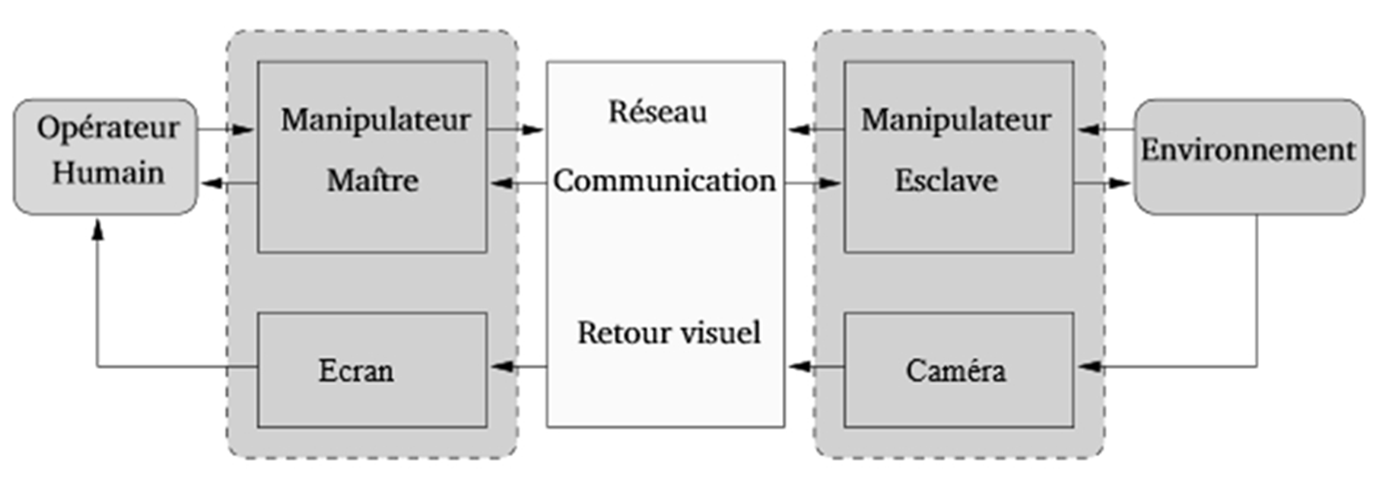
\includegraphics[width=\linewidth]{fig_00a}
%\textit{}
\end{center}


\section*{Modélisation de l’interface maître}

Ce mécanisme est constitué de 4 barres reliées par des liaisons pivots.

\begin{center}
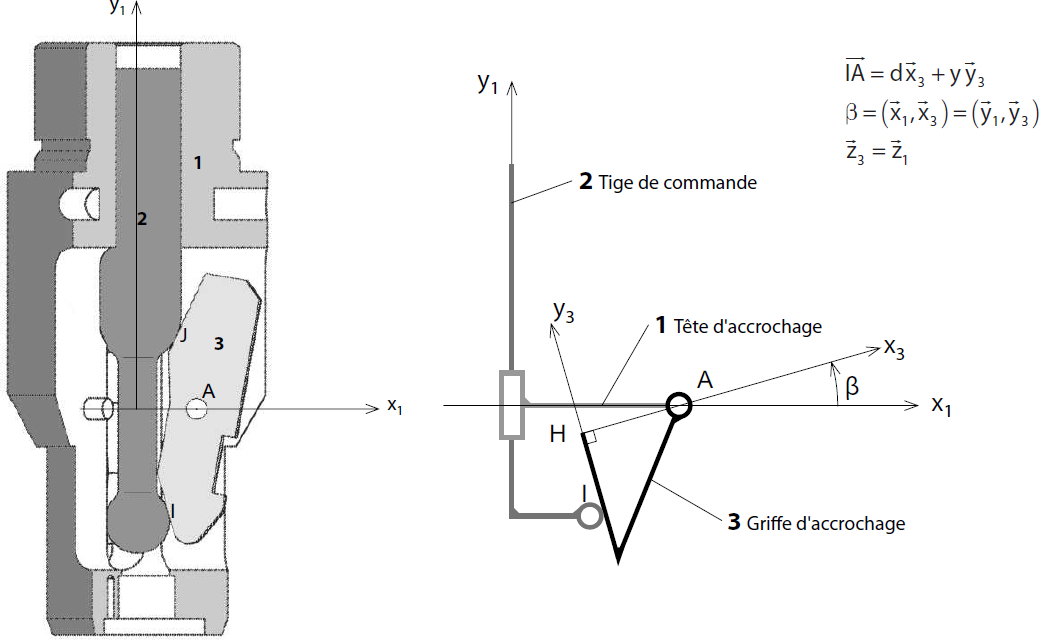
\includegraphics[width=\linewidth]{fig_01}
%\textit{}
\end{center}

\begin{obj}
Vérifier que les exigences « Amplitude déplacement » (id 1.2.1.1), « Mouvement
rectiligne » (id 1.2.1.2), « Linéarité déplacement » (id 1.2.1.3) peuvent être satisfaites par le mécanisme de HOEKEN.
\end{obj}


\begin{center}
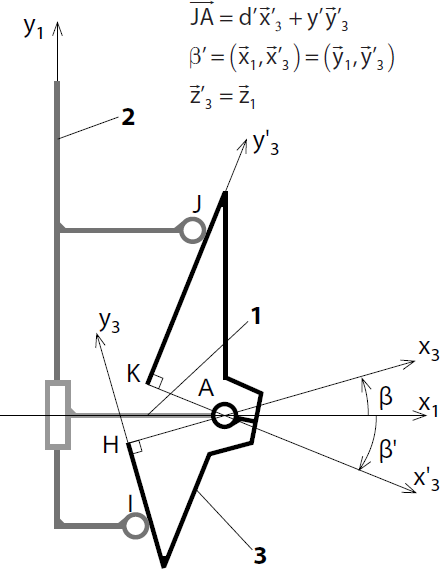
\includegraphics[width=\linewidth]{fig_02}
%\textit{}
\end{center}

\begin{itemize}
\item Solide $S_0$, repère $\rep{0}\repere{A}{x_0}{y_0}{z_0}$, $\vect{AB}=L_0\vect{x_0}$ avec $L_0 = \SI{50}{mm}$.
\item Solide $S_1$, repère $\rep{1}\repere{B}{x_1}{y_1}{z_0}$, $\vect{BC}=L_1\vect{x_1}$ avec $L_1 = \SI{25}{mm}$, $\theta_1=\angl{x_0}{x_1}=\angl{y_0}{y_1}$.
\item Solide $S_2$, repère $\rep{2}\repere{A}{x_2}{y_2}{z_0}$, $\vect{AD}=L_2\vect{x_2}$ avec $L_2 = \SI{62,5}{mm}$, $\theta_2=\angl{x_0}{x_2}=\angl{y_0}{y_2}$.
\item Solide $S_3$, repère $\rep{3}\repere{C}{x_3}{y_3}{z_0}$, $\vect{ED}=\vect{DC}=L_2\vect{x_3}$ avec  $\theta_3=\angl{x_0}{x_3}=\angl{y_0}{y_3}$.
\end{itemize}


\subparagraph{}\textit{En développant une fermeture géométrique en projection dans la base du repère $\rep{0}$, donner
une relation algébrique reliant les paramètres $L_0$, $L_1$, $L_2$, $\theta_1$ et $\theta_3$.}
\ifprof
\begin{corrige}~\\
\end{corrige}
\else
\fi

\subparagraph{}\textit{De même, exprimer le vecteur position du point $E$ ($\vect{AE}$) dans la base du repère $\rep{0}$ en fonction de $L_0$, $L_1$, $L_2$, $\theta_1$ et $\theta_3$.}
\ifprof
\begin{corrige}~\\
\end{corrige}
\else
\fi

La résolution analytique du système d’équations permettant d’obtenir le déplacement du
point $E$ en fonction de l’angle de rotation $\theta_1$ du moteur et des différentes longueurs du mécanisme
n’étant pas triviale, seuls les résultats d’une simulation numérique seront analysés.

\begin{center}
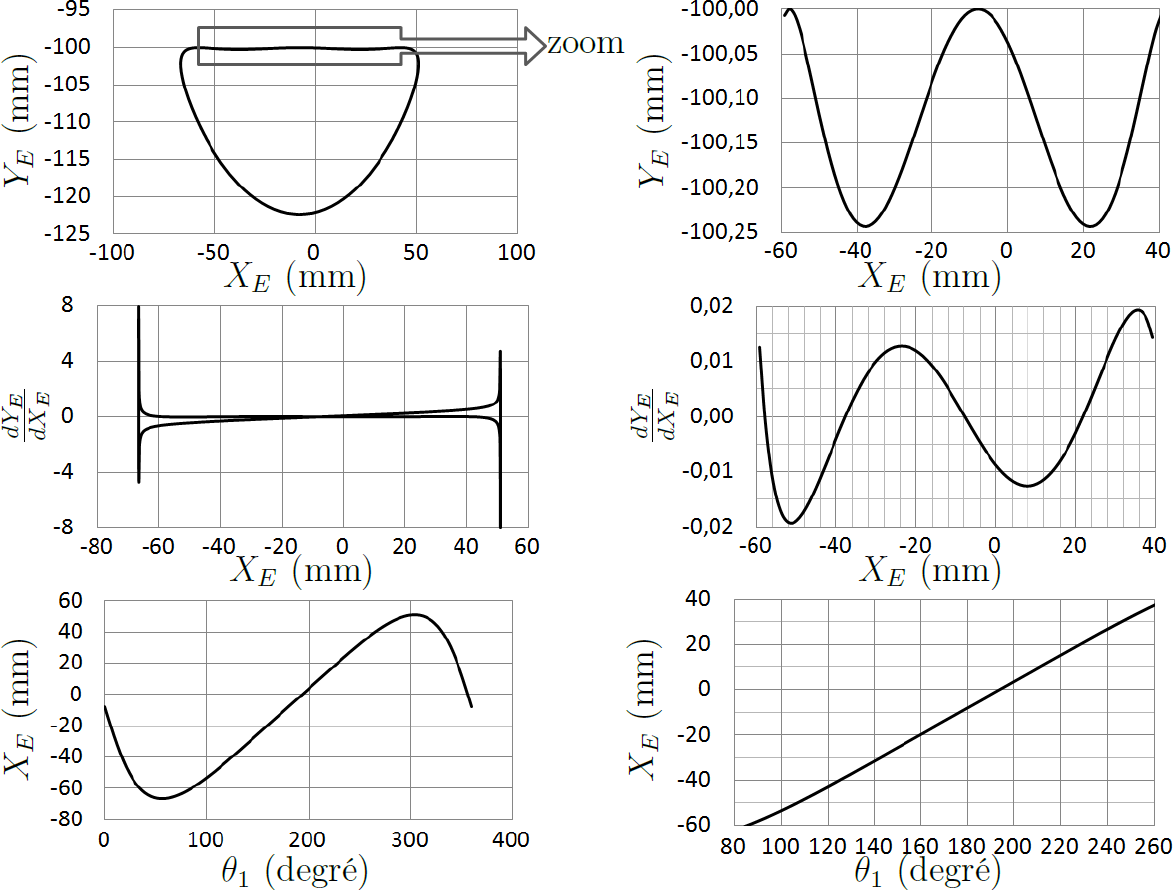
\includegraphics[width=\linewidth]{fig_03}
%\textit{}
\end{center}



\subparagraph{}\textit{Vérifier, à l’aide des figures précédentes, que le déplacement du point $E$ est compatible avec les
exigences « Amplitude déplacement » (id 1.2.1.1) et « Mouvement rectiligne » (id 1.2.1.2) sur
l’intervalle $X_E \in \left[-\SI{60}{mm}; \SI{40}{mm}\right]$.}
\ifprof
\begin{corrige}~\\
\end{corrige}
\else
\fi

\subparagraph{}\textit{Proposer, à partir de la dernière figure, une démarche permettant de vérifier l’exigence « Linéarité
déplacement » (id 1.2.1.3) sur l’intervalle $X_E \in \left[-\SI{60}{mm}; \SI{40}{mm}\right]$.}
\ifprof
\begin{corrige}~\\
\end{corrige}
\else
\fi


\section*{Modélisation de l’interface esclave}
\begin{center}
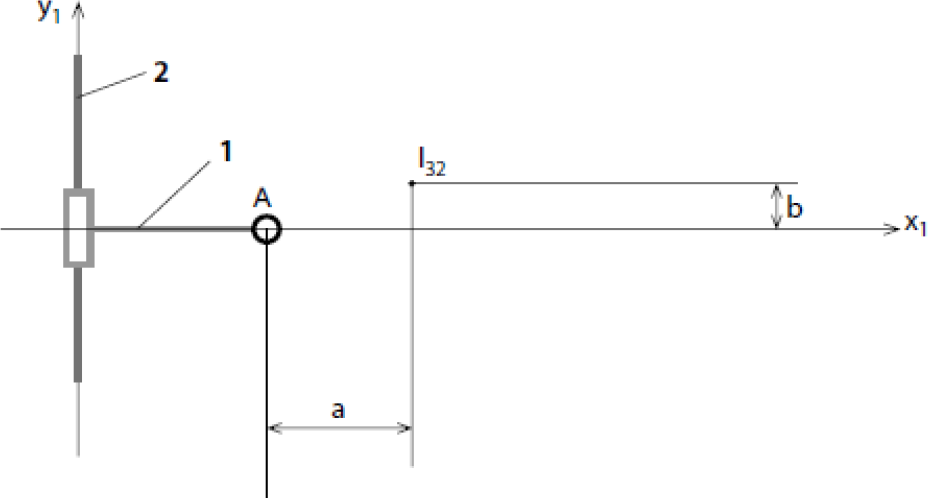
\includegraphics[width=.8\linewidth]{fig_04}
%\textit{}
\end{center}

\begin{center}
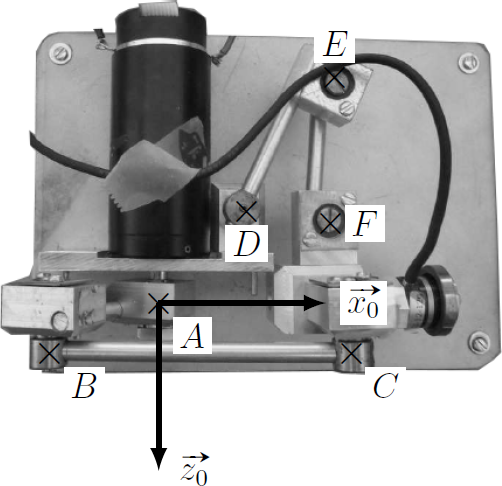
\includegraphics[width=.8\linewidth]{fig_05}
%\textit{}
\end{center}

\begin{center}
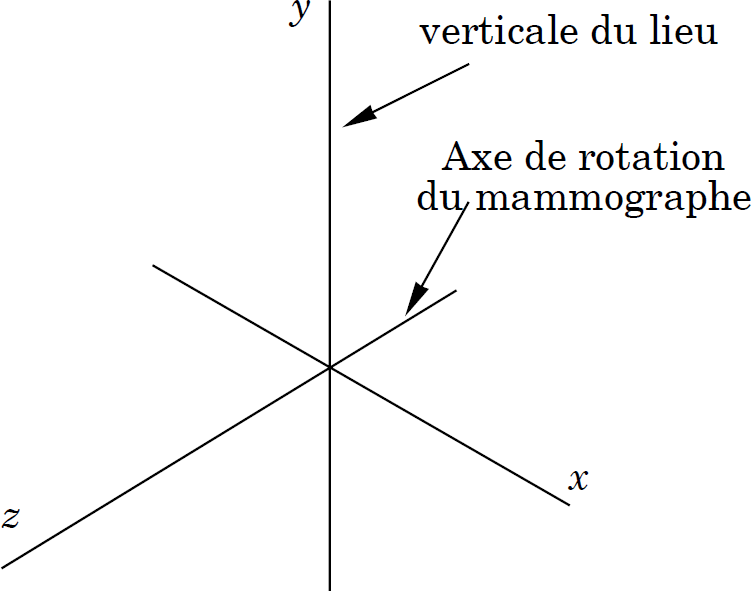
\includegraphics[width=\linewidth]{fig_06}
%\textit{}
\end{center}

\begin{center}
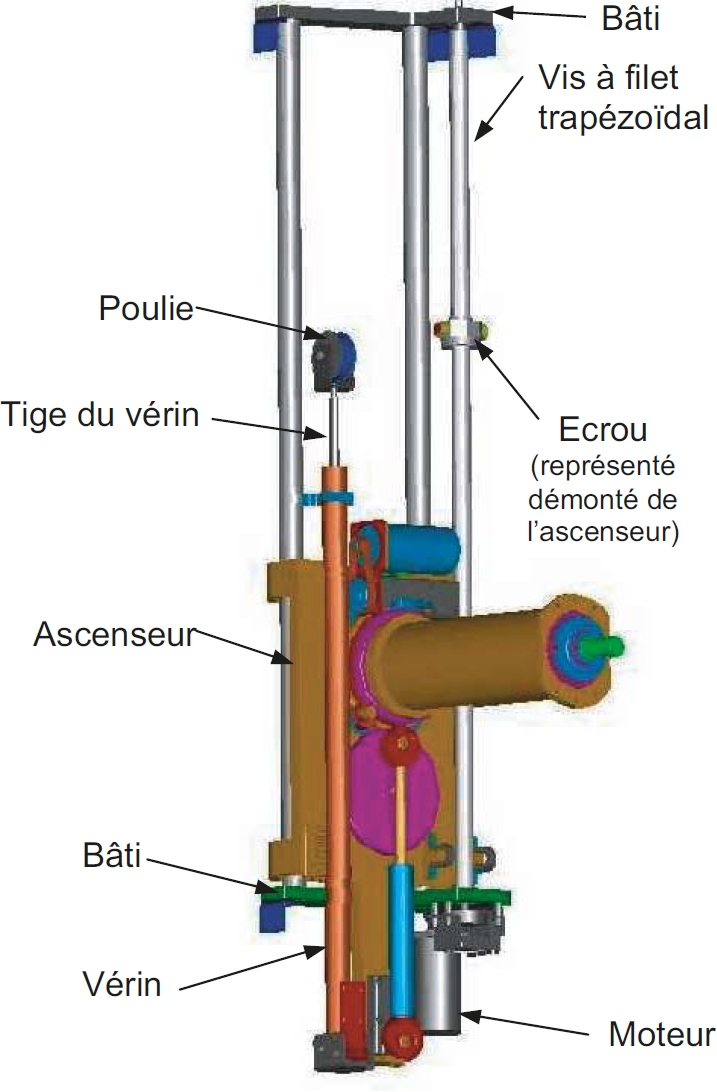
\includegraphics[width=\linewidth]{fig_07}
%\textit{}
\end{center}

\begin{obj}
Modéliser le comportement dynamique de l’interface esclave de façon à évaluer son
comportement au sein d’une boucle d’asservissement.
\end{obj}

On note $\torseurstat{T}{\text{mot}}{S_1}=\torseurl{\vect{0}}{C_m\vect{z}}{\forall P}$ l’expression, dans la base $\mathcal{B}_0$ du torseur de l’action mécanique exercée par le moteur sur le solide $S_1$ et
l’accélération de la pesanteur sera représentée par le vecteur $\vect{g} = -g \vect{y_0}$.

\subparagraph{}\textit{Tracer le graphe des liaisons du dispositif esclave. Donner le degré d’hyperstatisme de la modélisation de ce mécanisme.}
\ifprof
\begin{corrige}~\\
\end{corrige}
\else
\fi


\subparagraph{}\textit{Proposer une modification simple pour le rendre isostatique.}
\ifprof
\begin{corrige}~\\
\end{corrige}
\else
\fi


\subparagraph{}\textit{Montrer que le mouvement de $S_3/S_0$ ne peut être qu’une translation de direction $\vect{x_0}$.}
\ifprof
\begin{corrige}~\\
\end{corrige}
\else
\fi


\subparagraph{}\textit{En utilisant le théorème de l’énergie cinétique, déterminer l’équation de mouvement liant
les paramètres $C_m$, $\dot{\theta}_1$, $\ddot{\theta}_1$, $\dot{x}_s$, $\ddot{x}_s$, $f_v$, $M_3$ et $I_1$.}
\ifprof
\begin{corrige}~\\
\end{corrige}
\else
\fi


\subparagraph{}\textit{La relation géométrique liant les paramètres $x_s$ et $\theta_1$ n’étant pas triviale, on propose de la
linéariser autour du point de fonctionnement par l’expression $\theta_1(t)\simeq \alpha x_s(t)$ avec $\alpha=-\SI{30}{m^{-1}}$. En déduire l’équation différentielle liant les paramètres $C_m$, $\dot{x}_s$, $\ddot{x}_s$, $f_v$, $M_3$, $I_1$ et $\alpha$.}
\ifprof
\begin{corrige}~\\
\end{corrige}
\else
\fi


\subparagraph{}\textit{Donner, dans les conditions d’Heaviside et sous forme canonique, la fonction de transfert
modélisant le comportement dynamique du manipulateur esclave : $H(p) = \dfrac{X_s(p)}{C_m(p)}$ sachant que
$X_s(p) = \mathcal{L}\left[x_s(t)\right]$ et $C_m(p) = \mathcal{L}\left[c_m(t)\right]$. Faire l’application numérique.}
\ifprof
\begin{corrige}~\\
\end{corrige}
\else
\fi


\end{multicols}
